\chapter{Implementacja środowiska badawczego}
W niniejszym rozdziale przedstawiono proces implementacji środowiska badawczego pod kątem realizacji zdefiniowanych uprzednio scenariuszy badawczych. Spośród składowych omawianego procesu wyróznić należy: przygotowanie odmian topologii fizycznych środowiska w zależności od scenariusza badawczego, budowę interfejsów programowania aplikacji z wykorzystaniem porównywanych technologii, czy też zastosowanie mechanizmów pozwalających na weryfikację działania API w aspekcie programowania współbieżnego. Ponadto, zaprezentowana została konfiguracja dedykowanych porównywanym technologiom platform chmurowych, a także struktura elementów składających się na plan testowy, identyfikujący przeprowadzoną ewaluację w ramach narzędzia przeznaczonego do realizacji badań.    
\section{Realizacja topologii fizycznych}
W zależności od scenariusza badawczego, wykorzystywanego w kontekście przeprowadzonych ewaluacji, zbudowane zostały cztery odmienne warianty topologii fizycznych. Trzy spośród nich, tyczą się badań wykonywanych w środowisku lokalnym, natomiast czwarta z topologii, związana jest z obserwacją funkcjonowania interfejsów programowania aplikacji uruchomionych w obrębie określonych platform chmurowych.

W odniesieniu do każdej z topologii zbudowanej w środowisku lokalnym, zauważyć należy fakt zastosowania techniki rozproszonego testowania \textit{(ang. Distributed Testing)}, a także jasny podział odpowiedzialności w kontekście wszystkich wykorzystywanych urządzeń. Procedura zbierania obserwacji za każdym razem realizowana jest wewnątrz odpowiednio dostosowanej lokalnej sieci komputerowej cechującej się brakiem dostępu do sieci Internet. Ponadto, w obszarze połączonych ze sobą urządzeń systemu komputerowego, dezaktywowane zostały protokoły i usługi sieciowe generujące cykliczne komunikaty rozgłoszeniowe. Dzięki temu, wyeliminowano błędy pomiarowe o charakterze niedeterministycznym.

Odwołując się do topologii sieciowej zbudowanej w środowisku rozległym, zauważyć należy odmienny sposób pozyskiwania informacji o czasie przetwarzania pojedynczego żądania. W tym przypadku, wykorzystywane narzędzie pomiarowe służy jako generator żądań, jednakże czasy odpowiedzi na żądanie, zwrócone przez to narzędzie nie mogą być brane pod uwagę. Informacja o czasie przetwarzania żądania zostaje dostarczana bezpośrednio z interfejsu programowania aplikacji.

\subsection*{Konfiguracja pierwsza lokalnej topologii fizycznej środowiska badawczego}
\label{sec:lokalne-srodowisko-badawcze-ver-1}
Pierwsza spośród lokalnych topologii fizycznych środowiska badawczego zastosowana została w celu badania wpływu wykorzystania odmiennych systemów bazodanowych na wydajność interfejsów programowania aplikacji, a także w kontekście obserwacji istotności implementacji wzorca podziału odpowiedzialności.

W ramach niniejszej topologii, wyróżnić należy dwa interfejsy programowania aplikacji (tj. utworzone z wykorzystaniem technologii C\#/.NET oraz NodeJS/Express), komunikujące się z jednym z pięciu serwerów bazodanowych (tj. MySQL Server, PostgreSQL Server, Microsoft SQL Server, SQLite oraz MongoDB). W określonym momencie czasu, utrzymywane jest tylko jedno aktywne połączenie pomiędzy jednym z API a jednym z serwerów bazodanowych. Ponadto, wewnątrz lokalnej sieci komputerowej, wyróżnić należy urządzenie komunikacyjne którym jest router, a także trzy urządzenia końcowe. Pierwszy z hostów pełni rolę "dyrygenta testu", który dostarcza informacje o konfiguracji testowej bezpośrednio do dwóch pozostałych urządzeń końcowych. Te urządzenia z kolei, odpowiedzialne są za generowanie żądań zgodnie ze zdefiniowanym natężeniem, częstotliwością, a także czasem trwania ewaluacji. Każde z oddzielnych urządzeń fizycznych połączone jest z urządzeniem komunikacyjnym poprzez łącze przewodowe, o tej samej przepustowości (tj. 1Gb/s), a także identycznej kategorii przewodu (tj. kategoria 6).

Na ilustracji \ref{fig:topologia-1} przedstawiono schemat pierwszego wariantu lokalnej topologii fizycznej środowiska badawczego.

\begin{figure}[ht]
    \centering
     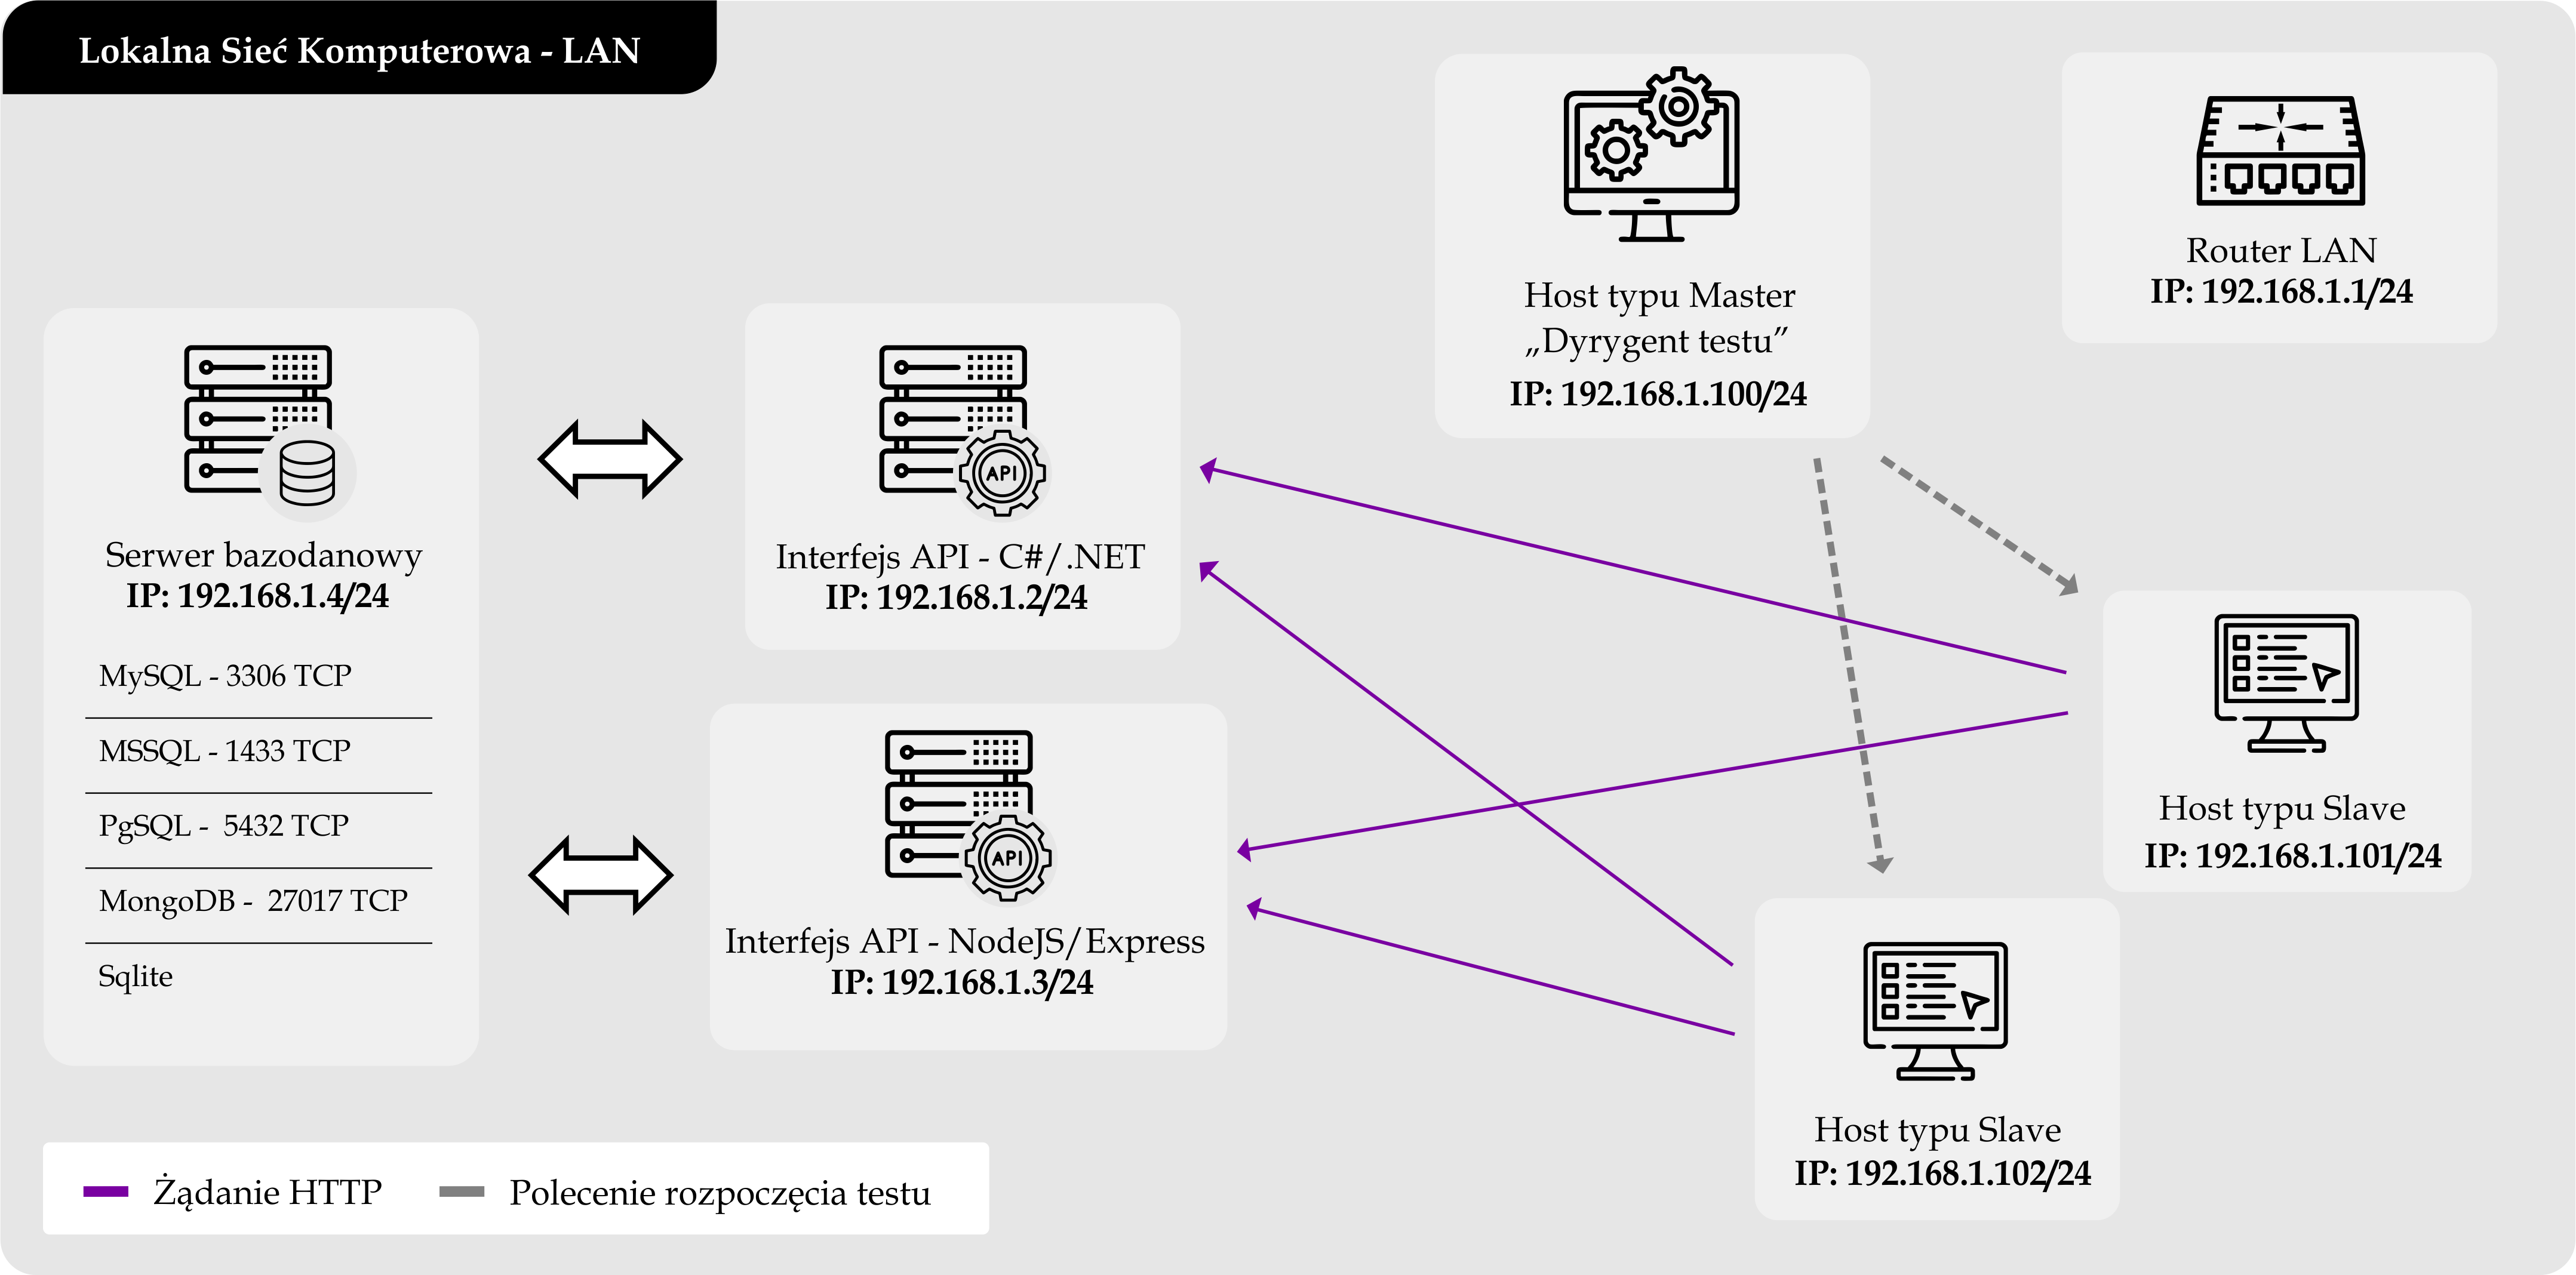
\includegraphics[width=\linewidth]{rys04/topologia-1.png}
    \caption{Konfiguracja pierwsza lokalnej topologii fizycznej środowiska badawczego}
    \label{fig:topologia-1}
\end{figure}

\subsection*{Konfiguracja druga lokalnej topologii fizycznej środowiska badawczego}
\label{sec:lokalne-srodowisko-badawcze-ver-2}
Druga topologia fizyczna środowiska badawczego, dotycząca ewaluacji w obrębie lokalnej sieci komputerowej, zbudowana została na potrzeby badań zaimplementowanych mechanizmów programowania współbieżnego, a także przechowywania odpowiedzi na żądania w ramach pamięci podręcznej.

W omawianej topologii wskazać należy dwa interfejsy programowania aplikacji, których implementacja dokonana została w porównywanych dwóch technologiach programistycznych. Obie usługi sieciowe, komunikują się z pojedyną instancją serwera bazodanowego - w przypadku badania pamięci cache, bądź też nie odwołują się do niego wcale - w przypadku badania efektywności operacji współbieżnych. Spośród urządzeń komunikacyjnych, wykorzystywanych do przeprowadzenia ewaluacji, wyróżnić należy jedno urządzenie typu Master (tzw. Dyrygent testu), a także jednego hosta typu Slave (tzw. generator żądań). Pierwszy z komputerów ma za zadanie przechowywać konfigurację wykonywanego badania, a także dostarczać komendy związane z rozpoczęciem i charakterystyką testu. Drugi host pełni rolę maszyny wytwarzającej i wysyłającej żądania protokołu hipertekstowego, zgodnie z koncepcją nakreśloną przez uzyskany plan ewaluacji. Wszystkie urządzenia znajdują się w obszarze pojedynczej, przewodowej lokalnej sieci komputerowej. Analogicznie do konfiguracji pierwszej, każde łącze przewodowe charakteryzuje się tym samym standardem oraz przepustowością.

Na ilustracji \ref{fig:topologia-2} przedstawiono schemat drugiego wariantu lokalnej topologii fizycznej środowiska badawczego.

\begin{figure}[ht]
    \centering
     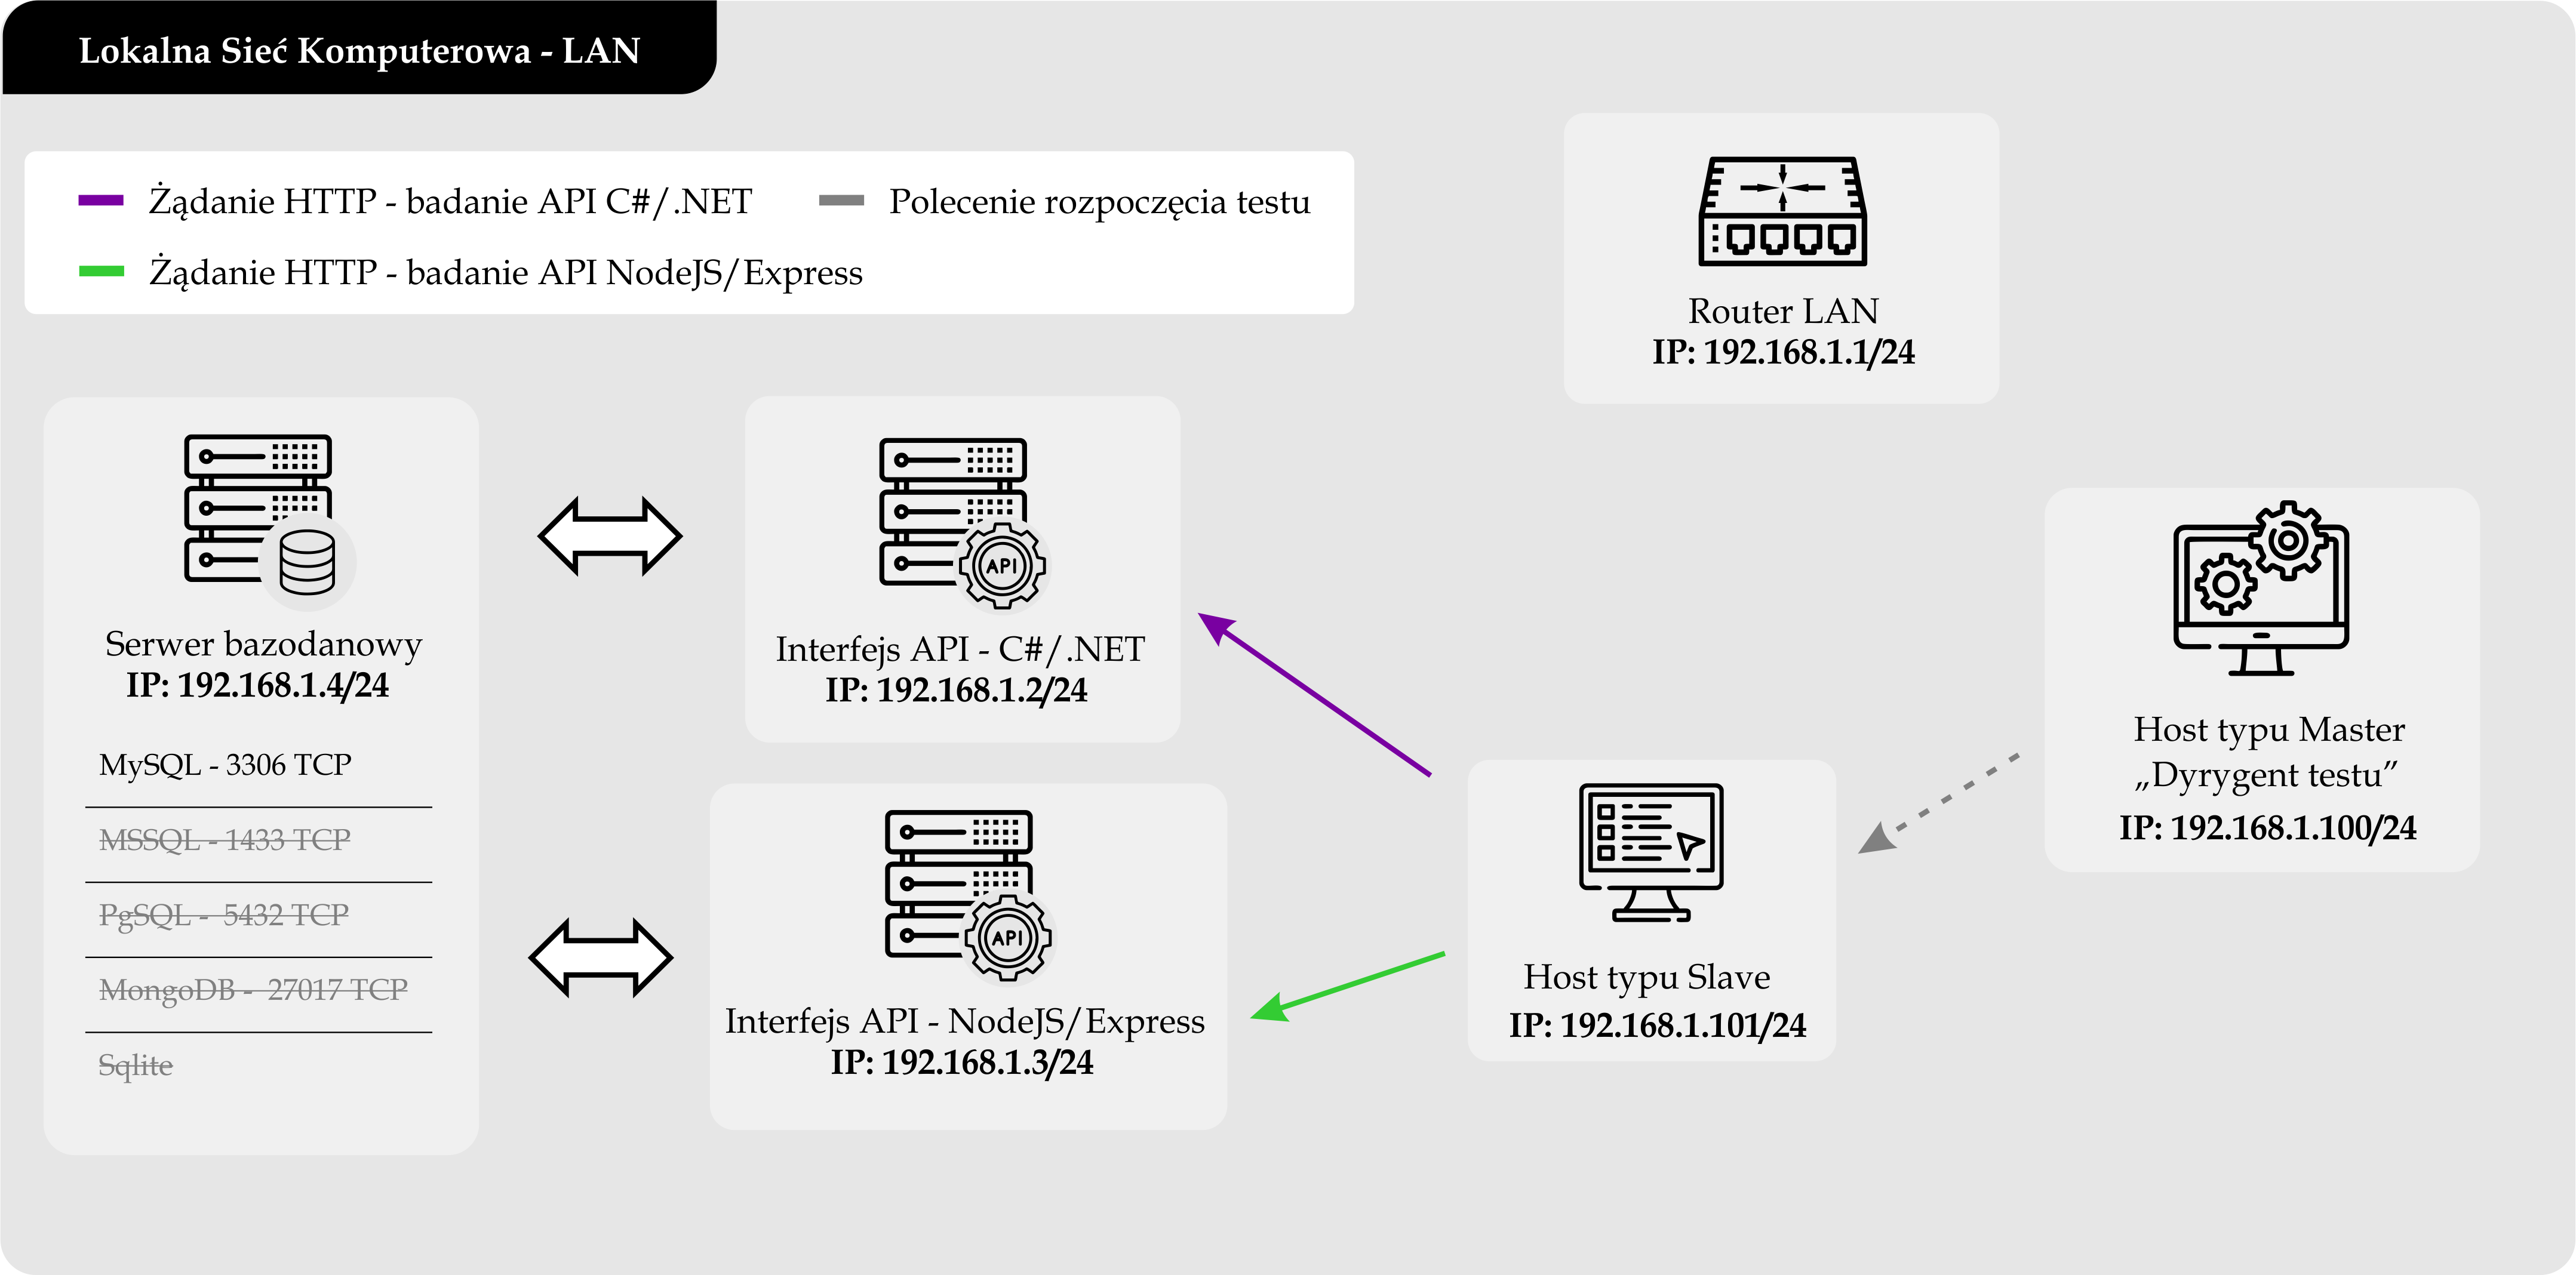
\includegraphics[width=\linewidth]{rys04/topologia-2.png}
    \caption{Konfiguracja druga lokalnej topologii fizycznej środowiska badawczego}
    \label{fig:topologia-2}
\end{figure}

\subsection*{Konfiguracja trzecia lokalnej topologii fizycznej środowiska badawczego}
\label{sec:lokalne-srodowisko-badawcze-ver-3}
Ostatnia z lokalnych topologii fizycznych środowiska badawczego przystosowana została w celu umożliwienia realizacji badań dotyczących wydajności obsługi operacji asynchronicznych.

W schemacie tym, zauważyć można wystąpienie trzech interfejsów programowania aplikacji. Analogicznie do topologii opisanych powyżej, dwa spośród trzech API zaimplementowane są w technologiach będących przedmiotem analizy tej pracy. Trzecia usługa sieciowa, służy do udostępniania zgromadzonych w niej danych, w związku z czym posiada ona tylko i wyłącznie punkty końcowe obsługiwane z wykorzystaniem metody GET. Punkty styku ostatniego z interfejsów dostarczają funkcjonalności pobierania danych o zróżnicowanym rozmiarze.

Ponadto, zbieżnie do konfiguracji pierwszej lokalnego środowiska badawczego, wyszczególnić możemy dwa urządzenia końcowe w roli generatorów żądań, oraz jednego hosta działającego w trybie "Dyrygenta testu". Należy podkreślić, że ewaluacje dotyczące każdej z technologii, zarówno w scenariuszach badawczych wykorzystujących tę, jaki i pozostałe topologie, wykonywane są w odrębnych chwilach czasu. Implikuje to fakt, że połączenie pomiędzy hostem badającym, interfejsem badanym, a także interfejsem pomocniczym jest aktywne tylko dla aktualnie badanego rozwiązania technologicznego.

Poza interfejsami programowania aplikacji oraz urządzeniami końcowymi wskażać należy urządzenie sieciowe, jakim jest przewodowy router LAN, który łączy wszystkie elementy topologii w ramach pojedynczej sieci LAN. Standard oraz przepustowość wykorzystywanych łączy pozostaje niezmienna względem pierwszej oraz drugiej z topologii fizycznych.

Na ilustracji \ref{fig:topologia-3} przedstawiono schemat trzeciego wariantu lokalnej topologii fizycznej środowiska badawczego.

\begin{figure}[ht]
    \centering
     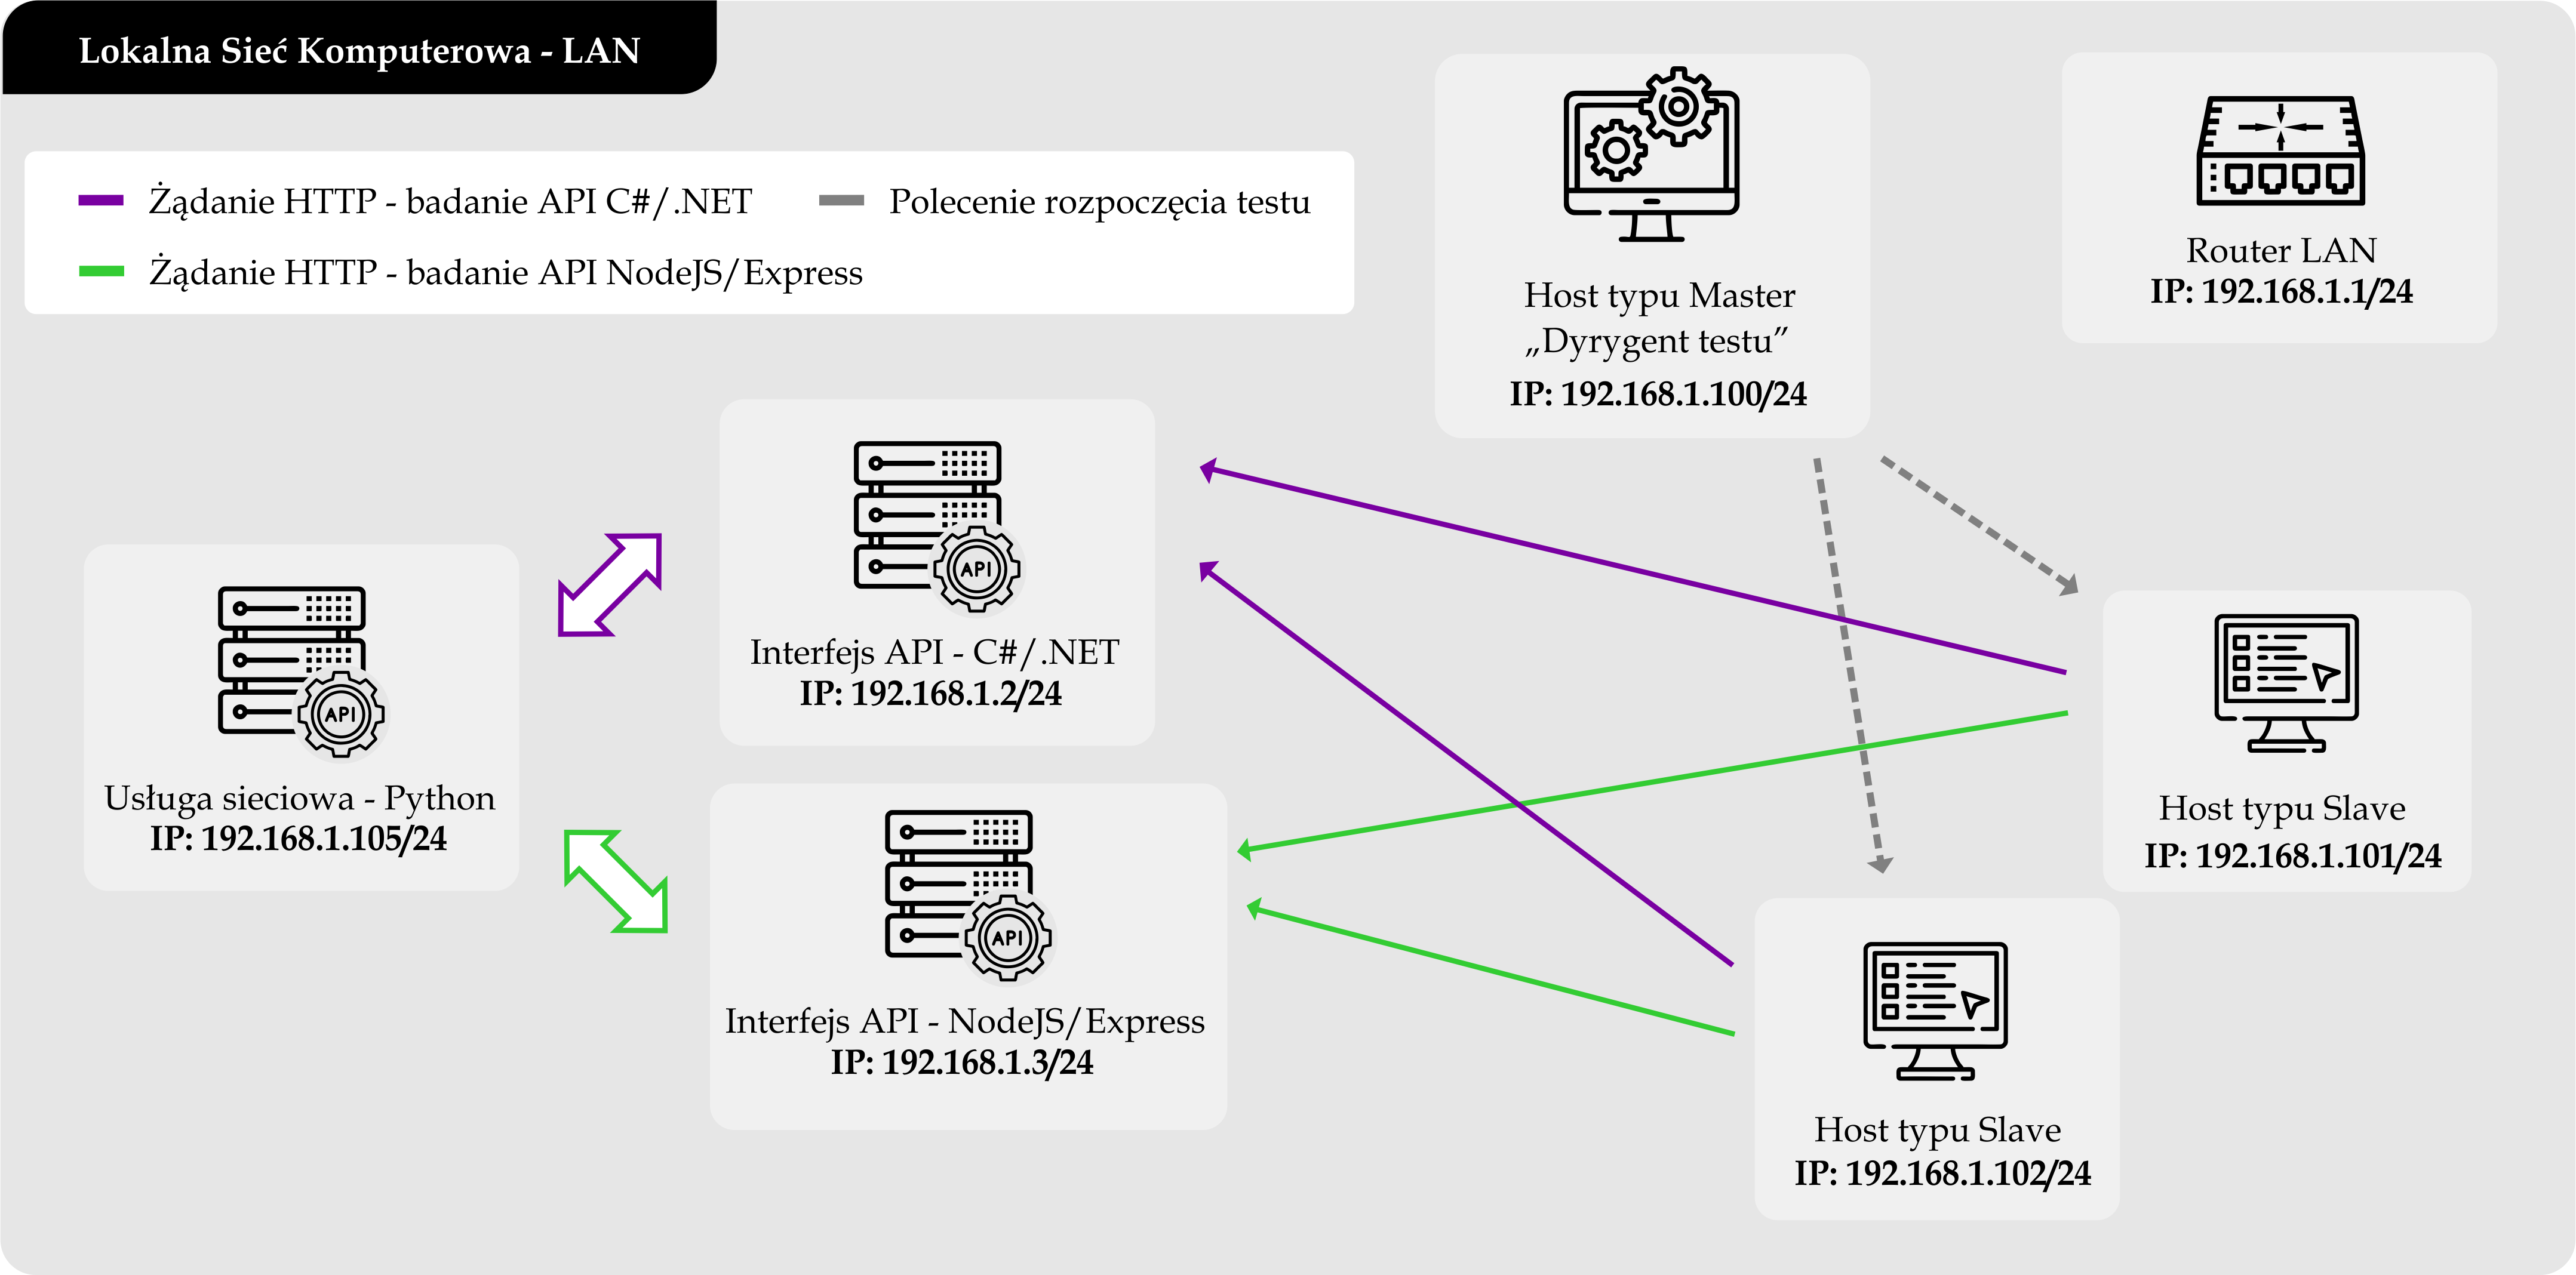
\includegraphics[width=\linewidth]{rys04/topologia-3.png}
    \caption{Konfiguracja trzecia lokalnej topologii fizycznej środowiska badawczego}
    \label{fig:topologia-3}
\end{figure}

\subsection*{Konfiguracja pierwsza rozległej topologii fizycznej środowiska badawczego}
\label{sec:rozproszone-srodowisko-badawcze-ver-1}
Konfiguracja topologii fizycznej dla rozproszonego środowiska badawczego, stworzona została w celu wykonania badań dotyczących efektywności działania interfejsów programowania aplikacji uruchamianych na odmiennych platformach chmurowych.

W tym przypadku, wyodrębnić należy dwa obszary, zawierające urządzenia w kontekście których przeprowadzana jest ewaluacja. Pierwszy obszar to lokalna sieć komputerowa, w której ulokowane zostały urządzenia końcowe odpowiedzialne za przechowywanie konfiguracji badania, a także generowanie żądań w kierunku API. W drugim obszarze zaś, nazwanym rozległą siecią komputerową uruchomione są platformy chmurowe, wewnątrz których działają interfejsy programowania aplikacji oraz serwery bazodanowe. Systemy internetowe zaimplementowane w odrębnych technologiach, przechowywane są na oddzielnych platformach chmurowych i nie są one ze sobą w żaden sposób skomunikowane. Zauważyć należy również fakt, że obie platformy chmurowe znajdują się w różnych lokalizacjach geograficznych. Stwierdzenia te, wymuszają modyfikację sposobu pozyskiwania pomiarów żądań, poprzez przeniesienie odpowiedzialności za wyliczenie czasu wykonywania operacji na interfejsy programowania aplikacji. Pomimo tego, niezbędnym jest posiadania urządzenia generującego żądania zgodnie z określoną charakterystyką. Dlatego też, wewnątrz obszaru lokalnego wskazać możemy dwa urządzenia końcowe, których rolą, podobnie do urządzeń końcowych zawartych we wszystkich poprzednich topologii fizycznych, jest generowanie żądań, oraz koordynowanie przeprowadzanego badania.

Na ilustracji \ref{fig:topologia-4} przedstawiono schemat pierwszego wariantu rozległej topologii fizycznej środowiska badawczego.

\begin{figure}[ht]
    \centering
     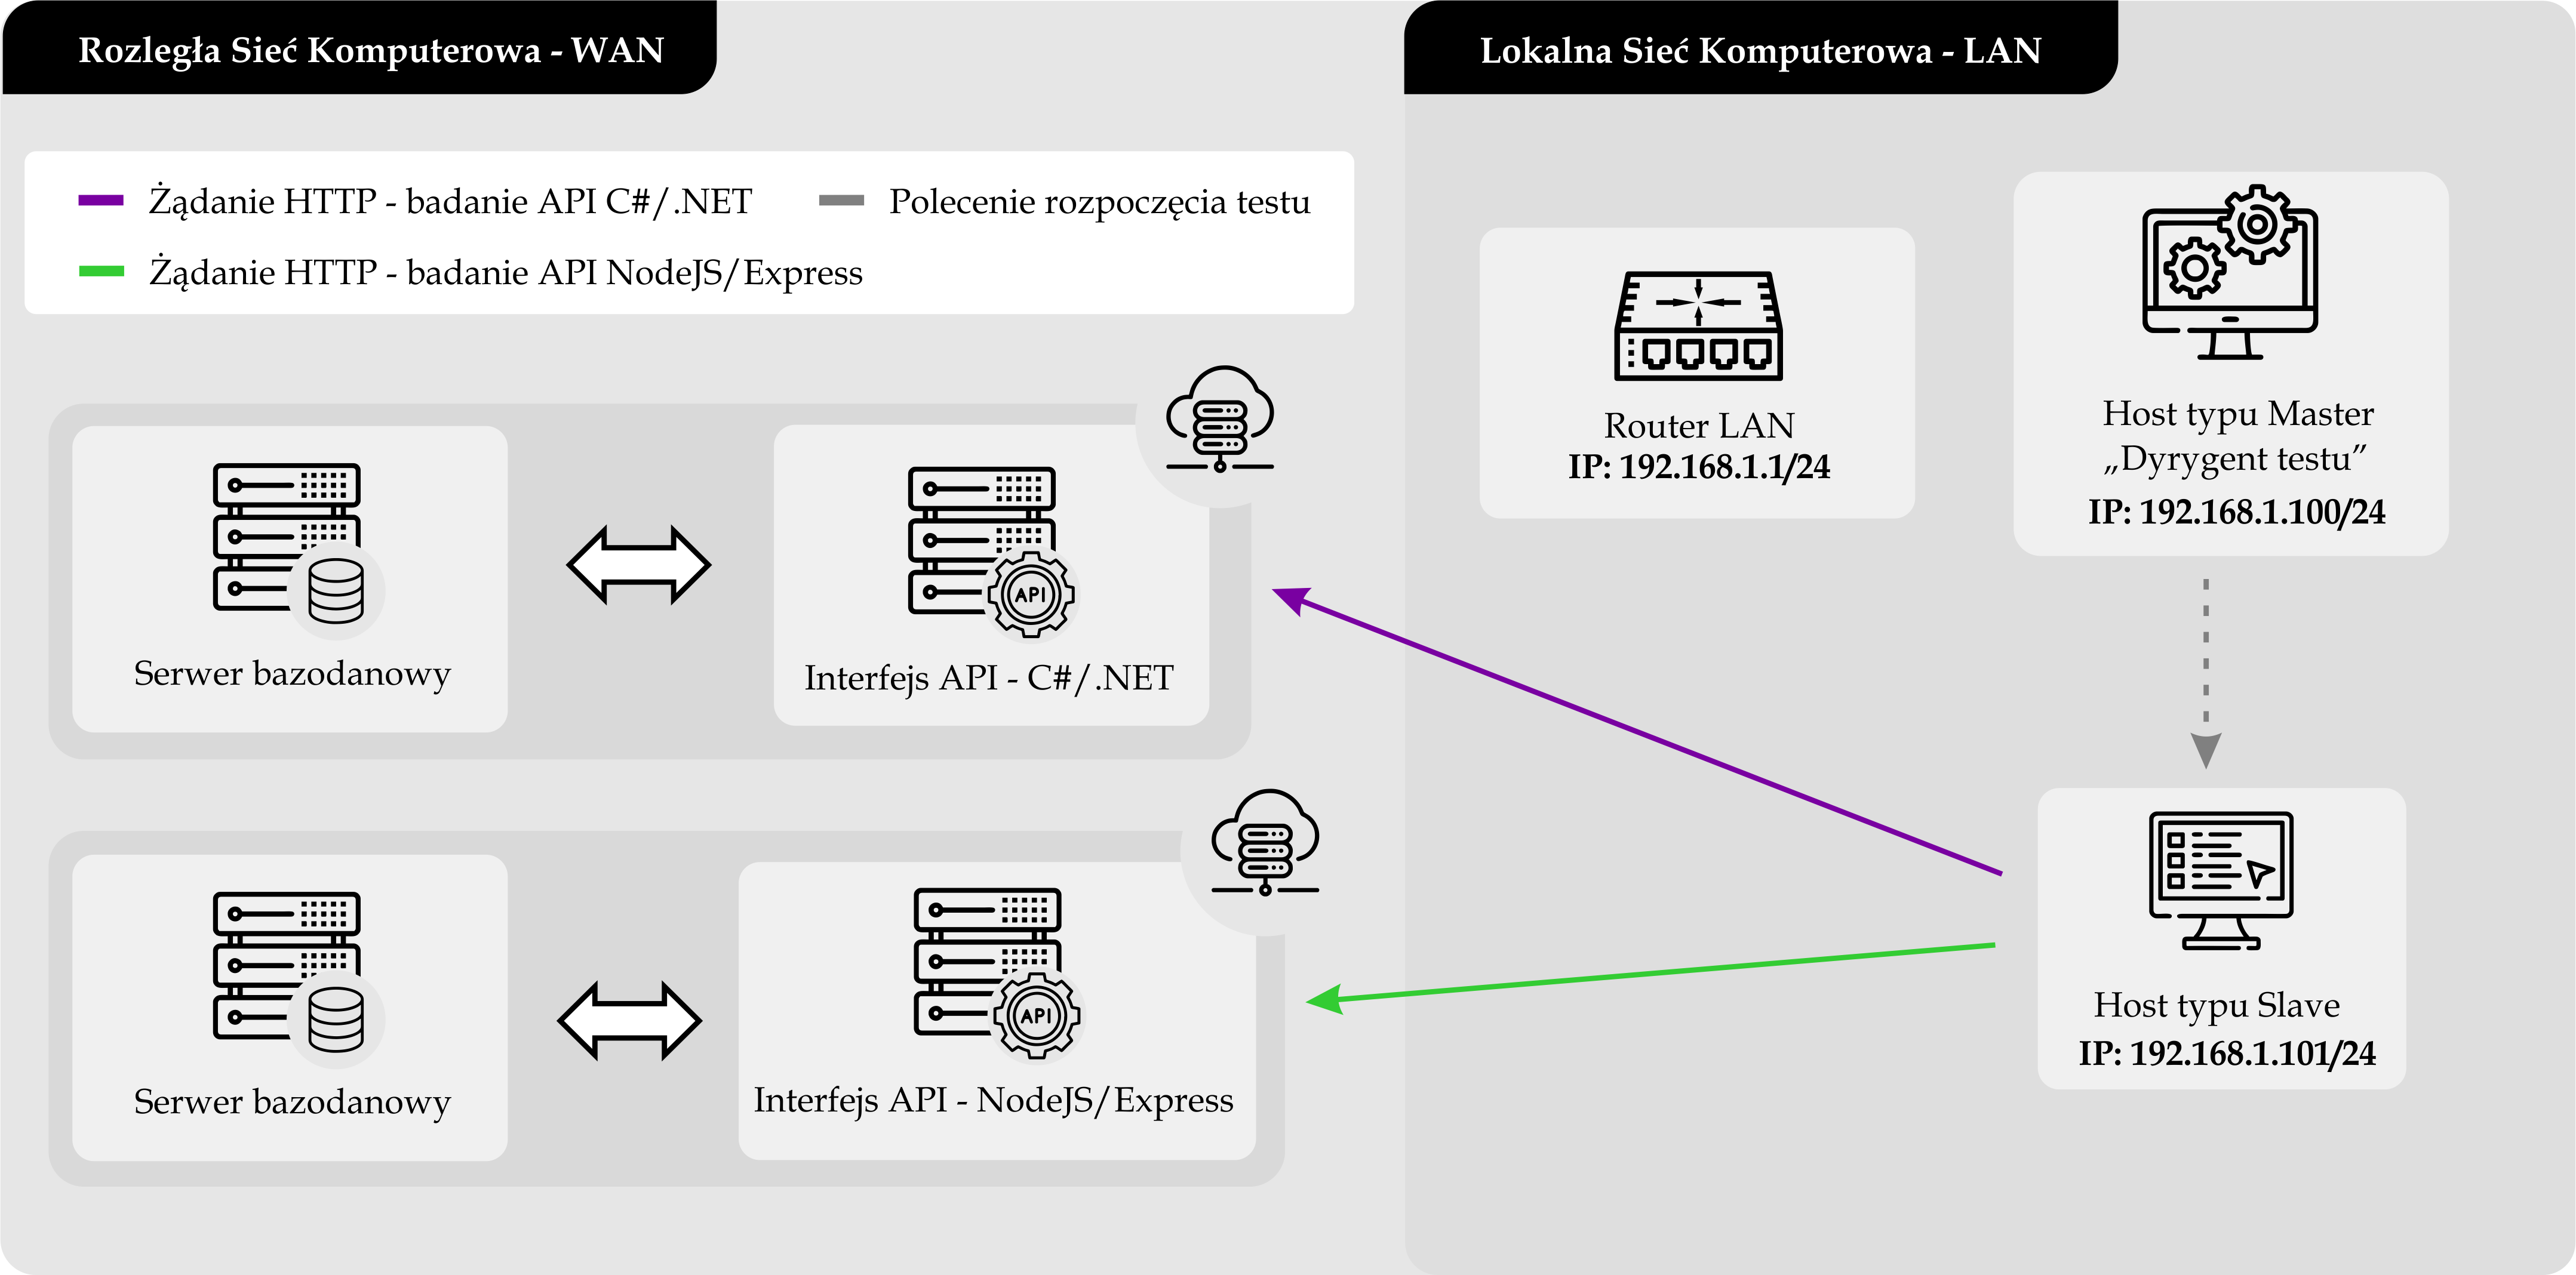
\includegraphics[width=\linewidth]{rys04/topologia-4.png}
    \caption{Konfiguracja pierwsza rozległej topologii fizycznej środowiska badawczego}
    \label{fig:topologia-4}
\end{figure}

\section{Budowa interfejsów programowania aplikacji}
\subsection*{Interfejs API realizujący operacje CRUD stworzony z wykorzystaniem technologii C\#/.NET}
\subsection*{Interfejs API realizujący operacje CRUD stworzony z wykorzystaniem technologii NodeJS/Express}
\subsection*{Algorytm metaheurystyczny dla symetrycznego problemu komiwojażera dostępny z poziomu punktu końcowego}
\subsection*{Mechanizm obsługi pamięci podręcznej z uwzględnieniem częstotliwości wywoływania punktów końcowych}
\subsection*{Implementacja wzorca projektowego CQRS z uwzględnieniem replikacji danych pomiędzy dwoma źródłami}
\section{Konfiguracja generycznych oraz dedykowanych platform chmurowych}
\section{Konfiguracja narzędzia do realizacji badań}


